\chapter{Mapeo de interiores mediante balizas bluetooth}
\label{cap:descripcionTrabajo}

En este capítulo explicamos el estudio realizado sobre el funcionamiento de los \textit{beacons} y su efectividad en el posicionamiento de interiores, concretamente en la Facultad de Informática de la UCM. Este trabajo de investigación ha sido muy satisfactorio ya que nos ha facilitado la toma de numerosas decisiones con las que elaborar una propuesta en resolución al mapeo del edificio y a la disposición concreta de las balizas que optimice el posicionamiento. 
%También ha contribuido a resolver algunos aspectos de la implementación que narraremos en el capítulo \ref{cap:diseñoeimplementación}.

\section{Estudio de la precisión del posicionamiento mediante los \textit{beacons}}

Una vez que hemos concluido, por las razones expuestas en la Sección \ref{sec:conclusionesposicionamiento}, escoger los \textit{beacons} como sistema de posicionamiento, vamos a realizar un estudio profundizando en los aspectos tecnológicos de estas balizas. El objetivo es comprender por completo su funcionamiento y comportamiento a la hora de medir distancias, es decir, cuánto rango tiene la señal bluetooth, con ayuda de qué función podemos recibir esta señal e interpretarla para determinar la distancia, qué margen de error presenta, en qué lugares es más aconsejable establecer las balizas para recibir mejor la señal y, por tanto, reducir el error, cómo de precisa es la distancia medida cuando el dispositivo móvil que recibe la señal bluetooth está en movimiento, etc. 

Los \textit{beacons} utilizados para este proyecto cuentan con una SDK (Kit de Desarrollo Software) propia de su marca (\textit{Kontakt}) en la que incluyen funciones ya implementadas que nos permiten conocer qué \textit{beacons} están en nuestro rango en un momento determinado y a cuántos metros están. Esta información se va actualizando cada cierto tiempo. También incluye un sistema de categorías en función de cómo de cerca o lejos esté un cierto dispositivo. Las categorías son las siguientes:

\begin{itemize}
	\item \textit{IMMEDIATE:} Si el dispositivo se encuentra a menos de $0,5$ metros.
	\item \textit{NEAR:} Si el dispositivo se encuentra entre $0,5$ y $3$ metros.
	\item \textit{FAR:} Si el dispositivo se encuentra a más de $3$ metros.
	\item \textit{UNKNOWN:} Si se ha perdido la señal del dispositivo.
\end{itemize}

Una vez descubiertas estas funciones y comprendido el código decidimos desarrollar dos pequeñas aplicaciones que sirviesen para un doble propósito. Por un lado, para tener una primera toma de contacto con el entorno de programación escogido, Android Studio, y con la incorporación de las funciones ofrecidas por la librería de \textit{Kontakt}. Y por otro, para analizar la precisión de la señal bluetooth (con y sin movimiento), concretar la posición óptima de los \textit{beacons} y desarrollar una primera idea sobre la estructuración de la información relevante del edificio en el mapeo y la implementación del código relativo al posicionamiento en el edificio. En las siguientes secciones presentamos las dos aplicaciones desarrolladas para estos fines.


\subsection{Aplicación \textit{miniapp}}
Esta aplicación constituye la primera toma de contacto con los \textit{beacons} y con el código de la SDK. Presenta una interfaz sencilla en la que aparece una tabla con las distintas categorías de proximidad para 3 balizas y, debajo, el espacio donde se indica el identificador de la baliza correspondiente. En el cuadro inferior aparecen dos botones muy intuitivos con los que el usuario puede interactuar con la app: Stop Scanning y Start Scanning. De esta manera, una vez que empieza el escaneo y las balizas se encuentran en el radio de detección, se incluyen los identificadores en cuestión y se colorea en verde la categoría de proximidad estimada en cada caso según corresponda. La lectura de los \textit{beacons} se actualiza cada 2 segundos, tiempo establecido de antemano. En la Figura \ref{fig:miniapp} podemos ver la interfaz descrita.

La idea que subyace al desarrollo de esta aplicación es introducirnos en Android Studio y manejar las funciones ofrecidas por la SDK de \textit{Kontakt}, de ahí que hayamos creado una primera interfaz con botones, cambios de color, cuadros de texto, etc. Una vez hecho esto, comprobamos que las funciones preestablecidas por la SDK funcionaban y realizamos distintas pruebas en una posición fija para establecer el grado de confianza que podíamos tener en las categorías de proximidad definidas por \textit{Kontakt}. El resultado fue muy positivo puesto que, en su mayoría, la categoría asignada se ajustaba a la realidad. Sin embargo, nos faltaba saber la precisión estricta de los \textit{beacons} al recibir la distancia exacta en metros. Por ello creamos una segunda aplicación que, aunque fuese menos visual desde el punto de vista de la interfaz, nos diese más información sobre los \textit{beacons} detectados.

\subsection{Aplicación \textit{cuadrantes\_v1}}
 \textit{Cuadrantes\_v1} es una aplicación austera. En ella aparece un gran cuadro de texto que ocupa practicamente la totalidad de la pantalla y dos botones que se sitúan en el cuadro inferior,  Stop Scanning y Start Scanning, a través de los cuales el usuario puede interactuar con la app. Su funcionamiento es sencillo e intuitivo: cuando el usuario pulsa Start Scanning comienza el escaneo de balizas y cuando una o varias entran en el radio de detección, la app plasma su información (identificador, distancia en metros y categoría de proximidad) en el cuadro de texto. Esta información se actualiza cada 2 segundos (tiempo configurable) hasta que el botón Stop Scanning es pulsado, momento en el cual cesa el escaneo. La Figura \ref{fig:cuadrantesv1} muestra la interfaz de la aplicación descrita.

Como mencionamos anteriormente, hemos creado esta aplicación con el fin de obtener más información sobre el error cometido a la hora de determinar la distancia en metros a la que se encuentran los \textit{beacons} (tanto si el dispositivo se encuentra parado como en movimiento), así como para estudiar cuales son los factores que alteran su señal. De esta manera podremos determinar los puntos claves donde colocar las balizas y abordar, tras ello, el mapeo del edificio. De ahí que el nombre de la aplicación sea \textit{cuadrantes\_v1} ya que, como veremos, los cuadrantes serán una pieza fundamental en el mapeo. A continuación exponemos las pruebas realizadas con ayuda de esta aplicación y algunas de las consecuencias derivadas de los resultados.

\begin{figure}
	\centering
	\subfloat[Interfaz de miniapp]{
	\label{fig:miniapp}
	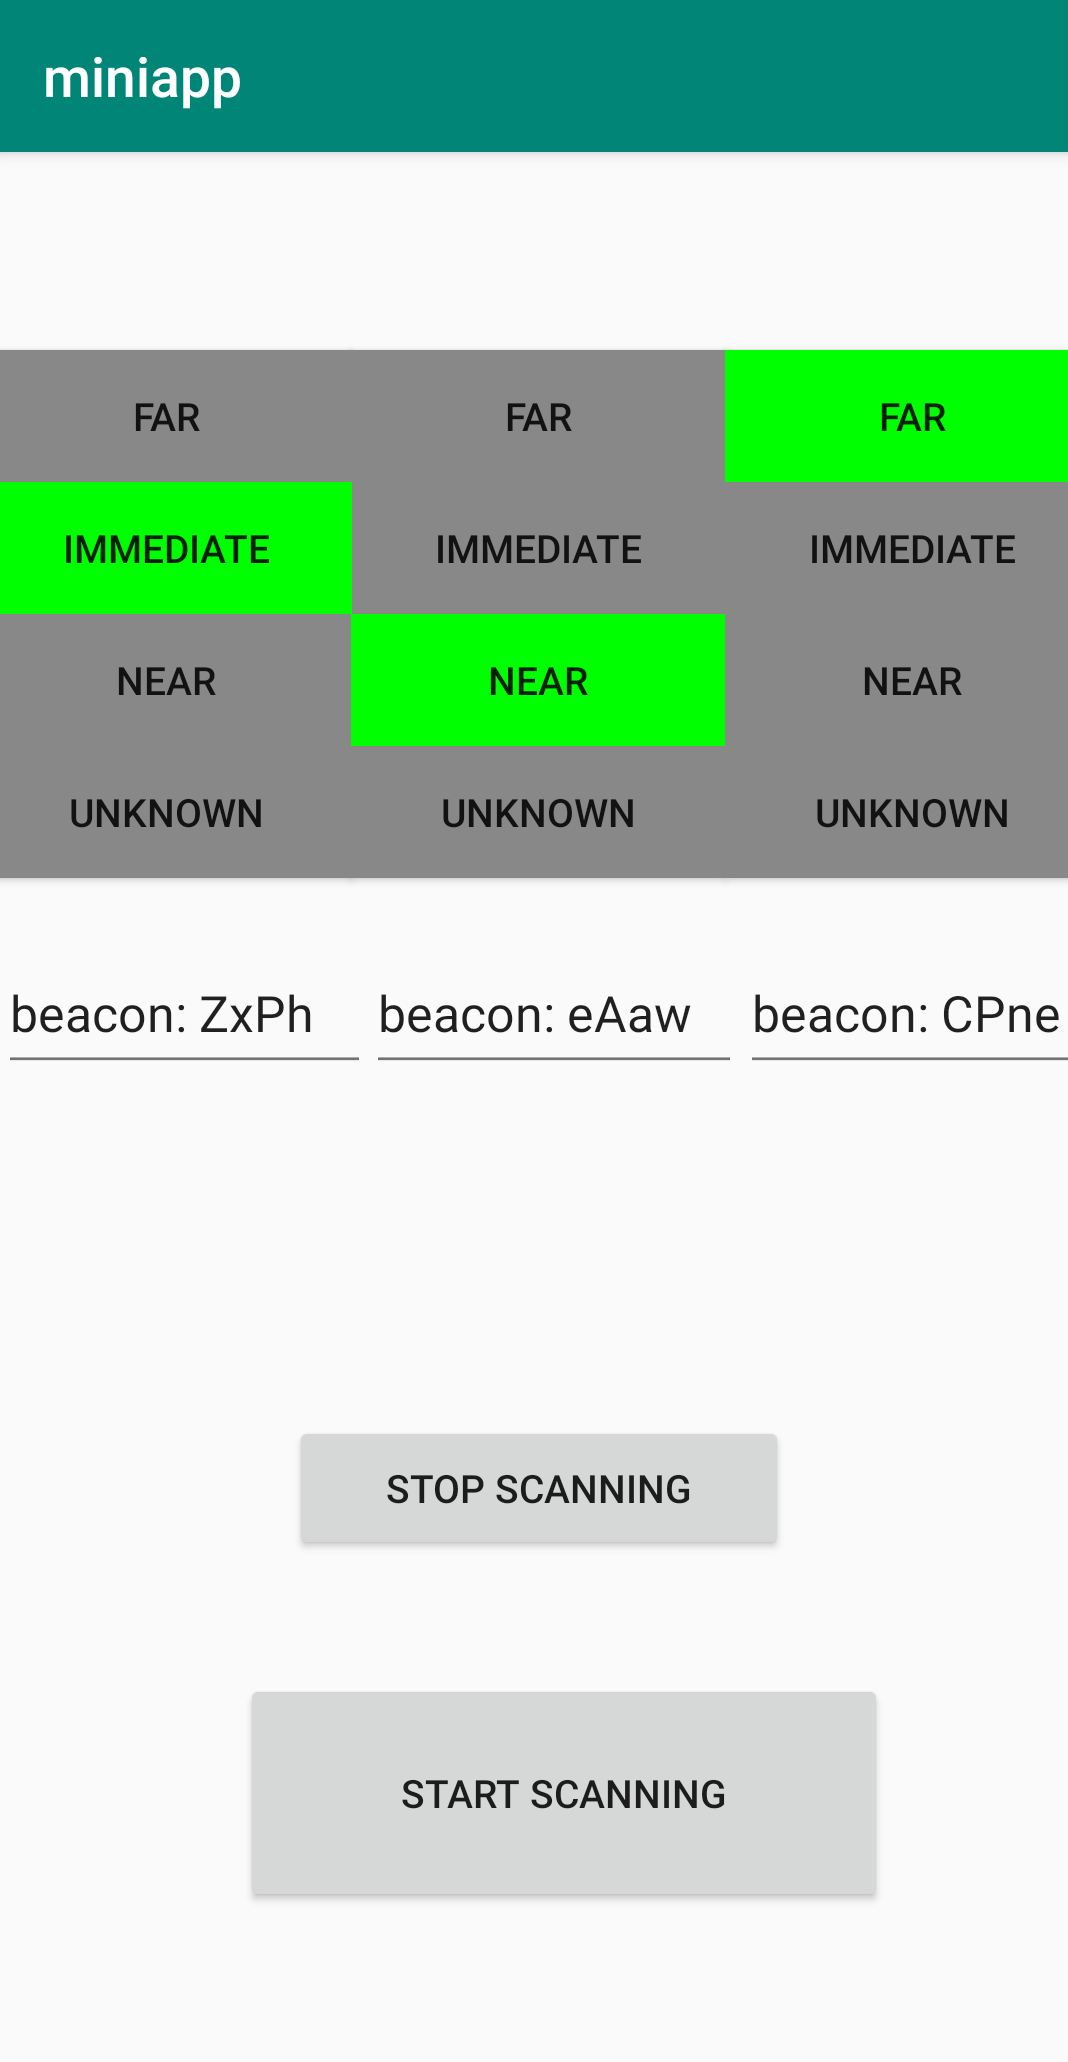
\includegraphics[width=0.3\textwidth]{Imagenes/Descripciondeltrabajo/miniapp}}
	\subfloat[Interfaz de cuadrantes\_v1]{
	\label{fig:cuadrantesv1}
	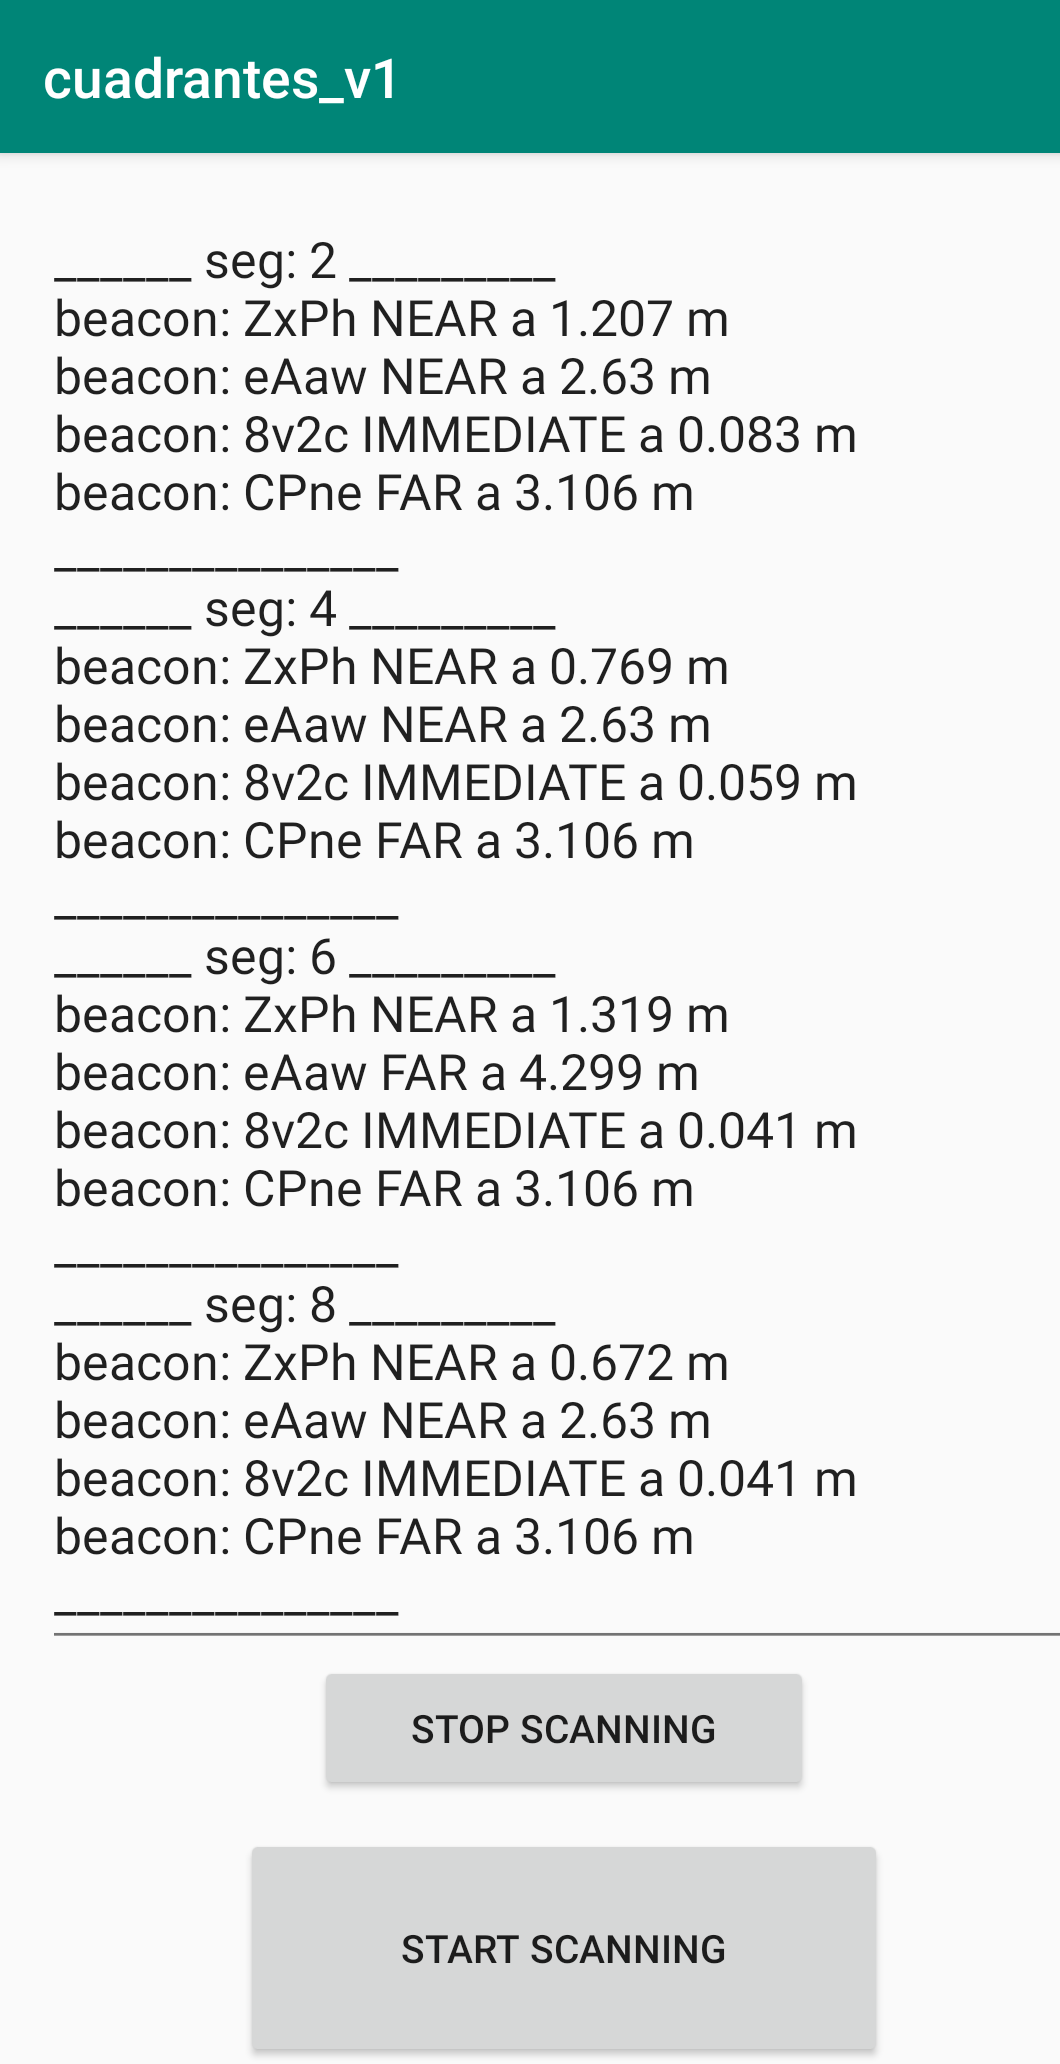
\includegraphics[width=0.3\textwidth]{Imagenes/Descripciondeltrabajo/cuadrantes_v1}}
	\caption{Aplicaciones auxiliares}
	\label{f:apps}
\end{figure}

\subsubsection{Pruebas con \textit{cuadrantes\_v1}}

Las primeras pruebas realizadas con la aplicación \textit{cuadrantes\_v1} han consistido en colocar tres \textit{beacons}, concretamente aquellos con identificadores CPne, 8v2c y eAaw, en distintos puntos de la Facultad de Informática y observar la distancia registrada desde un dispositivo móvil ubicado en un punto fijo. De esta manera, hemos podido medir el error cometido en cada caso y estimar las posibles interferencias. Para mostrar los resultados hemos creado tres gráficas que muestran la distancia a la que se detectan las balizas a lo largo del tiempo y la medida real a la que estaban situadas. 

En la Figura \ref{fig:dist_CPne} vemos las lecturas que nos ha proporcionado la aplicación \textit{cuadrantes v1} del \textit{beacon} con identificador CPne. En este caso, hemos realizado 4 estudios independientes marcados con distintos colores: azul -\textit{beacon} a 64cm, naranja -\textit{beacon} a 2m, gris -\textit{beacon} a 2,5m y amarillo -\textit{beacon} a 5 metros-. De esta gráfica concluimos que cuanto mayor es la distancia a la que se encuentra la baliza, véase la función amarilla (5m), más fluctúa la medida estimada convirtiéndose en un dato poco fiable. Correlativamente, a menor distancia menor error. Podemos ver que la función naranja (2m) es bastante fiel a la realidad, fluctúa en un intervalo de un metro a lo largo de toda la medición. Por último, el resultado de la gráfica azul (64cm) es bastante preciso, presenta un error despreciable durante toda la medición.

\begin{figure}[t]
	\centering
	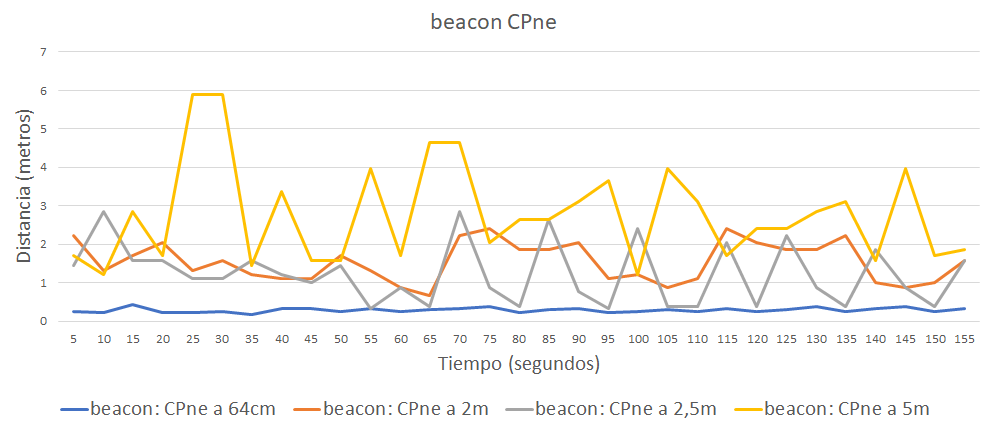
\includegraphics[width=0.8\textwidth]{Imagenes/Descripciondeltrabajo/dist_CPne}
	\caption{Gráfico con las distancias medidas al beacon CPne. }
	\label{fig:dist_CPne}
\end{figure}

En el caso de la Figura \ref{fig:dist_eAaw}, en la que se estima la distancia para el \textit{beacon} eAaw, pero usando distancias más pequeñas, el comportamiento es similar. En líneas generales, el valor medio estimado se corresponde con la distancia real a la que se encuentran las balizas. Sin embargo, en esta medición hemos contemplado una novedad que se ha repetido en numerosas ocasiones convirtiéndose en un patrón de comportamiento y es que durante los primeros segundos en los que arranca la aplicación, las estimaciones son menos precisas, dando lugar a picos importantes que más tarde se suavizan. 
\begin{figure}[t]
	\centering
	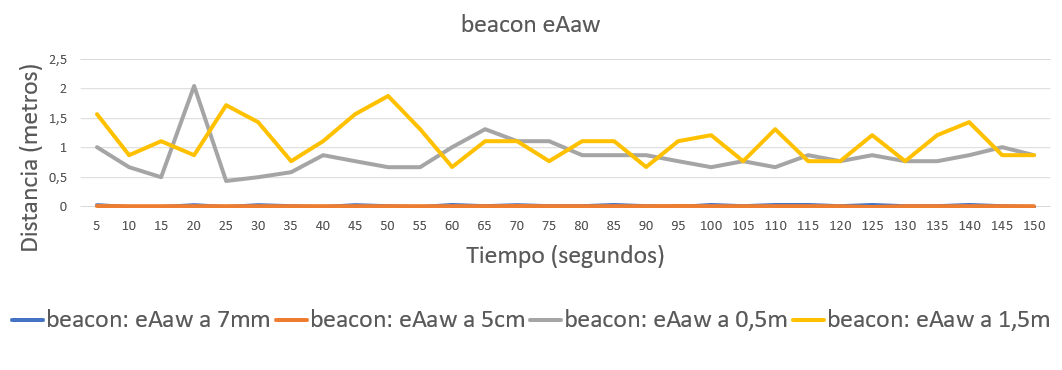
\includegraphics[width=0.8\textwidth]{Imagenes/Descripciondeltrabajo/dist_eAaw}
	\caption{Gráfico con las distancias medidas al beacon eAaw. }
	\label{fig:dist_eAaw}
\end{figure}

La Figura \ref{fig:dist_8v2c} recoge cuatro mediciones para el \textit{beacon} 8v2c, tres de ellas tomadas para una misma distancia (4m) y una a 64 cm. Observamos de nuevo que el error es despreciable cuando la baliza se encuentra muy próxima. Por el contrario, los valores que recogen las gráficas en las que el dispositivo se encuentra a 4m están muy por debajo de lo esperado, y solo una de ellas alcanza el valor real y en todas las direcciones. Este factor común nos reveló una alteración considerable de la intensidad de la señal por lo que empezamos a entrever que había factores en el entorno que la debilitan. Es por esto que la última gráfica, plasmada en la Figura \ref{fig:dist_conjunto}, hace referencia a una situación particular. Se trata de dos \textit{beacons} diferentes situados a la misma distancia uno encima del otro. El objetivo de este estudio era ver si uno de los factores que podía alterar la intensidad de señal era la presencia de otras balizas, y efectivamente como podemos observar, la intensidad de ambas señales es bastante más baja de lo esperado, prácticamente en ningún momento alcanzan el valor real. En este caso particular, el error es tolerable ya que los \textit{beacons} están situados a muy poca distancia pero sí nos advierte de que la señal bluetooth es sensible a interferencias provocadas por otros \textit{beacons} del entorno, lo cual hemos de tener muy presente a la hora de determinar la ubicación de los beacons a lo largo de la facultad para no colocarlos demasiado próximos. En la Sección \ref{sec:Interferencias} del Capítulo \ref{cap:estadoDeLaCuestion} se han expuesto algunas de las causas de las interferencias.
\begin{figure}[t]
	\centering
	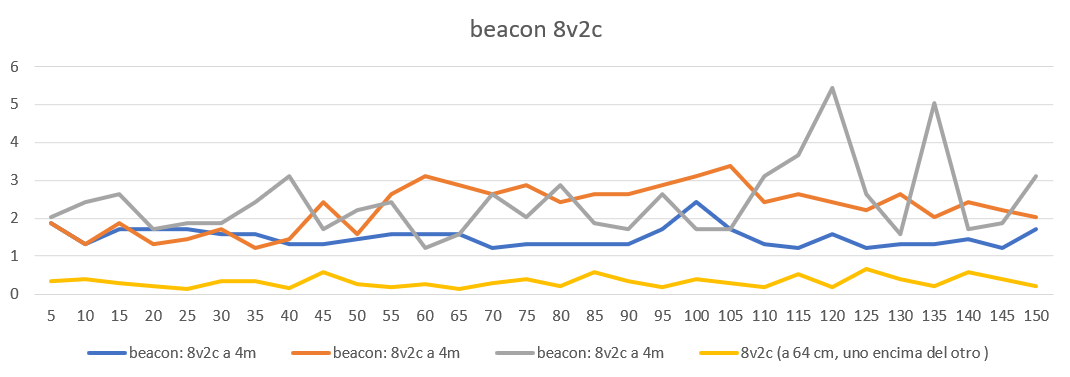
\includegraphics[width=0.8\textwidth]{Imagenes/Descripciondeltrabajo/dist_8v2c}
	\caption{Gráfico con las distancias medidas al beacon 8v2c. }
	\label{fig:dist_8v2c}
\end{figure}
\begin{figure}[t]
	\centering
	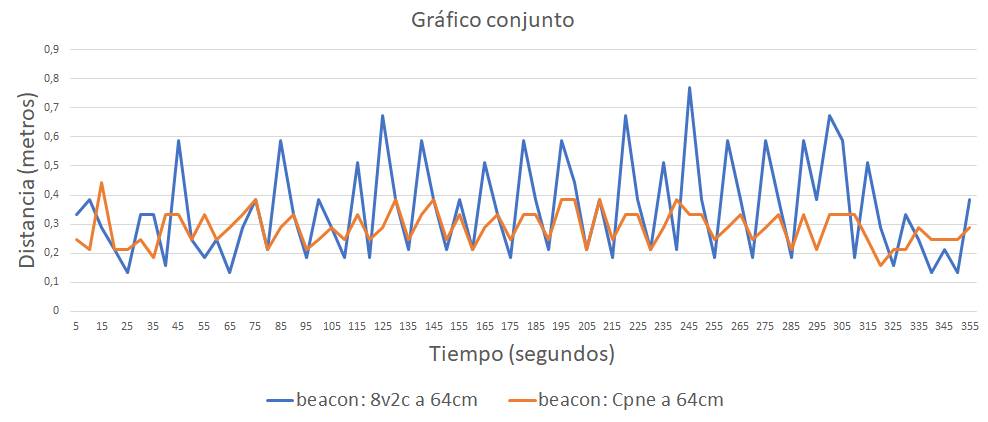
\includegraphics[width=0.8\textwidth]{Imagenes/Descripciondeltrabajo/dist_conjunto}
	\caption{Gráfico de los beacons 8v2c y CPne superpuestos. }
	\label{fig:dist_conjunto}
\end{figure}

\subsection{Conclusiones de la precisión de los \textit{beacons}}
\label{sub:conclusiones_posicionam}
Con todos estos resultados hemos decidido que para el posicionamiento utilizaremos el dato del \textit{beacon} más cercano ya que es la medida más fiable (por estar a menos metros del dispositivo) y consideraremos que el usuario se encuentra en las inmediaciones de dicho \textit{beacon}. En la Sección \ref{sec:mapeo} especificaremos la asociación realizada entre ``las inmediaciones de un \textit{beacon}'' y un punto concreto de la Facultad de Informática.

Con esta idea hemos desarrollado una primera aplicación de prueba que además de captar el \textit{beacon} más próximo al usuario emite un pitido a mayor o menor frecuencia según su categoría de proximidad. Esta app se llama \textit{pruebaSonido} y presenta la misma estética que \textit{cuadrantes\_v1}. Su funcionamiento es sencillo: al iniciar el escaneo capta el \textit{beacon} más cercano y lo fija. Tras ello, actualiza su información (concretamente, la distancia registrada y la categoría de proximidad) y pita a una frecuencia u otra según la distancia a la que se encuentre el \textit{beacon} (cuanto más cerca, el pitido es más rápido y se ralentiza a medida que la baliza está a mayor distancia). La actividad continúa hasta que el botón Stop Scanning es pulsado. Al igual que en \textit{cuadrantes v1} la información sobre las balizas detectadas queda plasmada en el cuadro de texto.

El objetivo de \textit{pruebaSonido} no es solo generar un primer código que seleccione el \textit{beacon} más cercano sino también llevar a cabo las primeras pruebas de estimación de la distancia a la que se encuentran las balizas en movimiento. Estos resultados han sido muy similares a los obtenidos estáticamente: la estimación sigue siendo más precisa cuanto más próxima está la baliza del dispositivo que la rastrea. Sin embargo, hay que ajustar el tiempo de actualización del escaneo si se quiere caminar a mayor velocidad (para que la aplicación reaccione en tiempo real y no sufra retrasos). Tras diversas pruebas hemos concluido que 2s es una medida óptima en lo que a nuestra aplicación concierne ya que nuestros usuarios, al presentar discapacidad visual, no caminan especialmente rápido. Por otro lado, esta aplicación nos ha servido también para incluir sonidos. Esto puede parecer insignificante, pero si nos paramos a pensarlo hay muchísimos sonidos que tenemos asociados con determinadas acciones, situaciones y/o aplicaciones que sin darnos cuenta nos guían en su uso y nos proporcionan la seguridad de que estamos utilizándola bien o la certeza de que tenemos que rectificar. Este recurso es indispensable en nuestra app ya que nuestros principales usuarios no podrán ver la aplicación.


\begin{figure}[t]
	\centering
	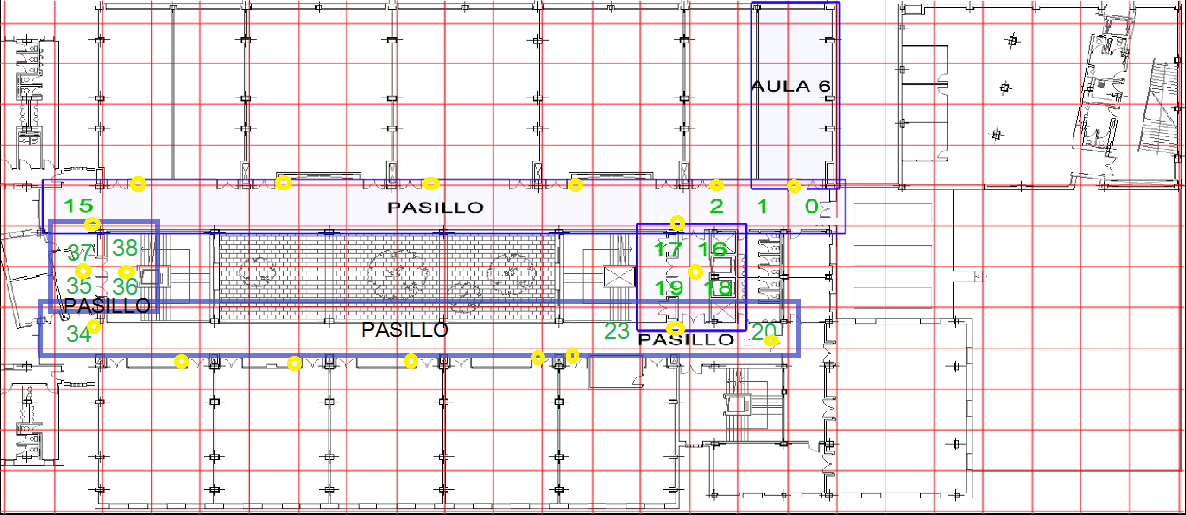
\includegraphics[width=1\textwidth]{Imagenes/Descripciondeltrabajo/mapaplanta1_cuadrantes}
	\caption{Primera versión del mapeo de la primera planta de la Facultad de Informática.}
	\label{fig:cuadrantesP1_v1}
\end{figure}



\section{Mapeo del edificio de la Facultad de Informática}
\label{sec:mapeo}

Para el mapeo de la Facultad de Informática nos hemos apoyado fundamentalmente en el proyecto de TFG \textit{Generador interactivo de instrucciones de guía sobre plataformas móviles} \citep{TFGguia}. De este, hemos reutilizado el sistema de estructuración basado en plantas que a su vez se dividen en cuadrantes con identificador único, lo que facilita determinar la planta en la que nos encontramos.
Originariamente, cada cuadrante se correspondía con nueve baldosas aproximadamente, tanto en el largo como en el ancho, y los cuadrantes se juntaban formando estancias (pasillos, aulas, etc.). De esta manera quedaban definidas cada una de las plantas del edificio y así empezamos definiendo también las nuestras. Sin embargo, sus cuadrantes contaban con dos números asociados que hacían referencia a las coordenadas sureste y noroeste que empleaban en el posicionamiento mediante triangulación Wi-Fi. Este es el primer cambio que hemos implementado ya que carecen de sentido en un posicionamiento como el nuestro, que se basa en puntos de decisión. En su lugar, debemos asociar los \textit{beacons} a los cuadrantes correspondientes. Para ello, empezamos determinando que no todos los cuadrantes tendrían una baliza asociada, sino que serían solo aquellos que tuviesen un punto de decisión. En la Figura \ref{fig:cuadrantesP1_v1} mostramos el primer acercamiento al mapeo de la planta 1 con los cuadrantes originales (en rojo), su identificador (en verde), algunas estancias (en azul) y la posición final de los \textit{beacons} (en amarillo). La disposición de los \textit{beacons} y su evolución hasta alcanzar la posición final se explicará y justificará adecuadamente en la Sección \ref{sec:medicionesbeacons}.


\begin{figure}[t]
	\centering
	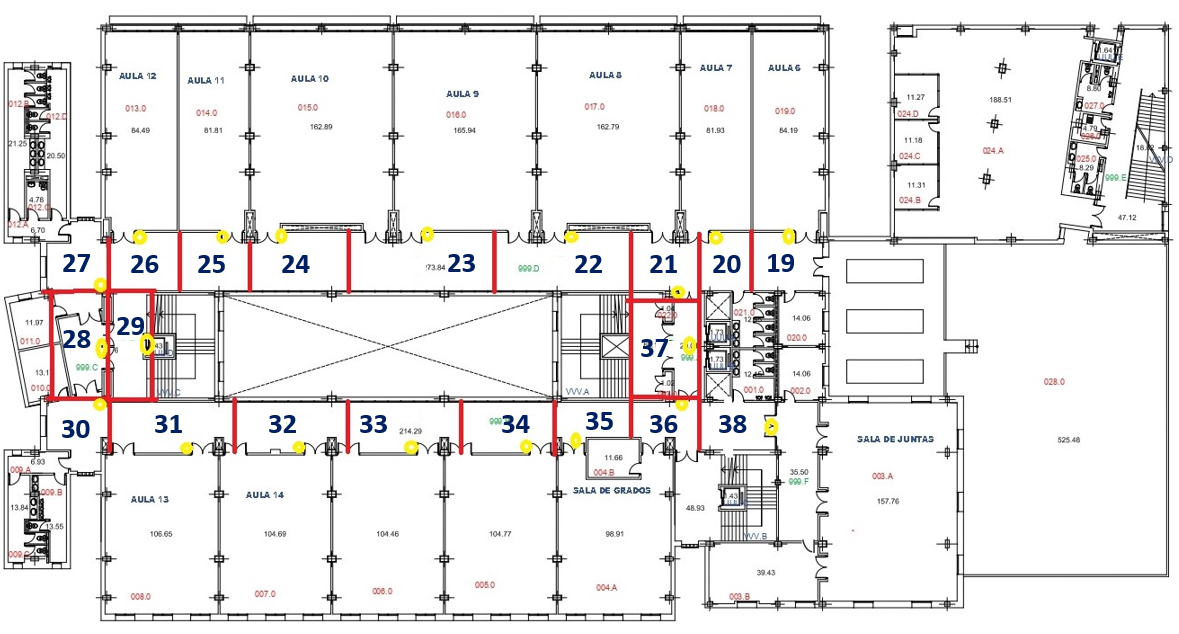
\includegraphics[width=1\textwidth]{Imagenes/Descripciondeltrabajo/mapeoPlanta1}
	\caption{Versión final del mapeo de la primera planta de la Facultad de Informática.}
	\label{fig:cuadrantesP1_v3}
\end{figure}


Como nuestro posicionamiento se fundamenta en el \textit{beacon} más cercano, hemos considerado que el usuario se encuentra en el cuadrante asociado a dicho \textit{beacon}, de esta manera es como hemos relacionado la frase ``encontrarse en las inmediaciones de un \textit{beacon}'' con un punto del mapa. Sin embargo, por este mismo motivo, aquellos cuadrantes que no tienen asociada ninguna baliza bluetooth carecen de interés ya que no hay manera de detectarlos y saber si el usuario se encuentra en ellos. Es por esto que el siguiente cambio ha sido juntar ciertos cuadrantes formando unos nuevos más grandes. En la Figura \ref{fig:cuadrantesP1_v3} encontramos la versión final del mapeo, en la que solo permanecen los cuadrantes con baliza. Además podemos observar que también hemos suprimido los cuadrantes de las aulas, sala de juntas, etc. esto se debe a que nuestra aplicación no ofrece una guía dentro de estas estancias sino que funciona como guía de puerta a puerta. Por ello, en lugar de tener cuadrantes que se unen formando estancias hemos realizado el cambio a cuadrantes que se agrupan en plantas.

\begin{figure}[t]
	\centering
	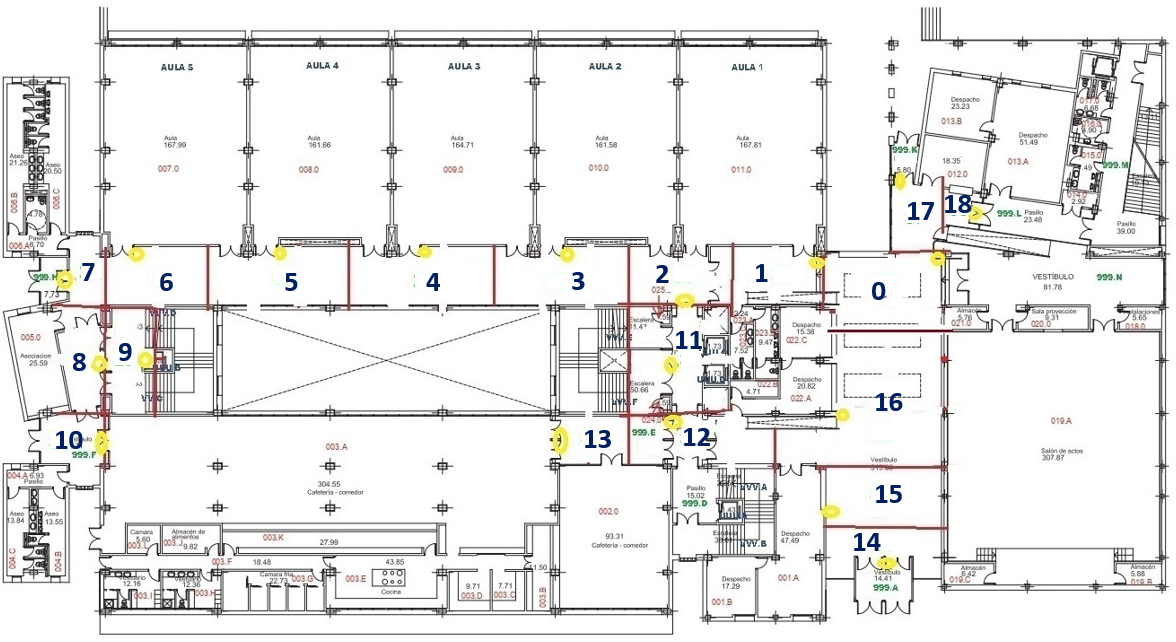
\includegraphics[width=1\textwidth]{Imagenes/Descripciondeltrabajo/mapeoPlantaBaja}
	\caption{Mapeo de la planta baja de la Facultad de Informática, incluyendo la numeración de los cuadrantes y las posiciones de los \textit{beacons}.}
	\label{fig:cuadrantesPbaja}
\end{figure}

La novedad más importante que incluye nuestro proyecto con respecto a los trabajos predecesores en este aspecto es el mapeo de la planta baja (ver Figura \ref{fig:cuadrantesPbaja}) y la conexión de unas plantas con otras a través de los cuadrantes en los que se encuentran los ascensores y escaleras de manera que sea viable incluir rutas de una a otra.



\section{Mediciones y distribución de los \textit{beacons} en la Facultad de Informática}
\label{sec:medicionesbeacons}

Ahora que hemos superado la primera barrera tecnológica y tenemos una idea más clara del mapeo, nos disponemos a dar el siguiente paso hacia la resolución del problema del posicionamiento. En este apartado proponemos una posible disposición de los \textit{beacons} en la Facultad de Informática de la UCM, para ello explicamos qué puntos hemos empezado considerando como puntos de decisión y su evolución hasta formar la disposición final que aparece en las Figuras \ref{fig:cuadrantesP1_v3} y \ref{fig:cuadrantesPbaja} como consecuencia de una serie de mediciones.

Antes de nada vamos a definir qué es un punto de decisión: Los puntos de decisión son aquellos lugares en los que el usuario requerirá la siguiente instrucción bien porque se ha creado incertidumbre (intersección de caminos), porque ha pasado mucho tiempo de la última instrucción (recta muy larga) o bien porque ha llegado al destino y requiere confirmación. Los puntos de decisión que hemos considerado en la Facultad de Informática son: los destinos (aulas, cafetería, biblioteca, conserjería, secretaría, salón de actos, sala de juntas, sala de grados, etc.), las intersecciones de caminos, los ascensores y escaleras, y las puertas de entrada o salida del edificio.

En la Figura \ref{fig:medidasPPrimera} mostramos visualmente los puntos de decisión que inicialmente hemos considerado (círculos rojos) en uno de los pasillos principales de la primera planta y los puntos desde los cuales hemos llevado a cabo las mediciones (cruces verdes). Esta estructura se repite tanto en la misma planta como en la planta baja por lo que las decisiones tomadas han sido las mismas y la evolución de la ubicación de los \textit{beacons} hasta ocupar su posición final ha sido copiada sin realizar pruebas distintas.

De manera análoga, en la Figura \ref{fig:medidasPBaja} mostramos la ubicación inicial de los \textit{beacons} en la zona del \textit{hall} de la planta baja y los puntos desde los cuales se han realizado las mediciones. El objetivo de todas estas mediciones es conocer la ubicación óptima de los \textit{beacons} para que a nuestro paso cerca de ellos, la distancia registrada sea lo más precisa posible y no sufra muchas interferencias. Este estudio debe ser especialmente exhaustivo en las zonas más delicadas, como las intersecciones o los lugares en los que se acumulan varios puntos de interés y que por ente, son más susceptibles a sufrir interferencias procedentes de otros \textit{beacons}. En la Sección X se pueden ver los resultados de estas mediciones. 
%RAQUEL DICE QUE PONGAMOS AQUI LOS RESULTADOS-BELENCHU!


\begin{figure}[t]
	\centering
	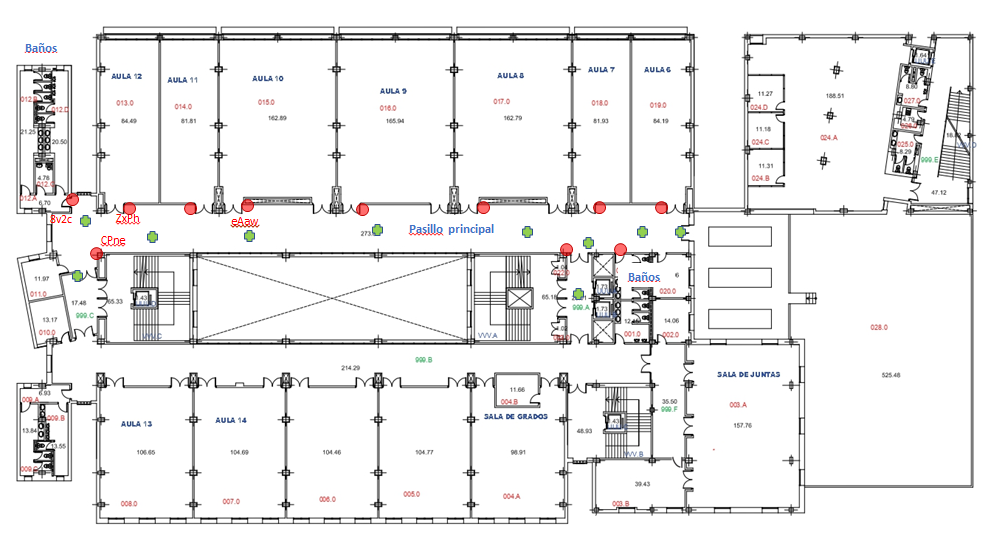
\includegraphics[width=1\textwidth]{Imagenes/Descripciondeltrabajo/mapa_mediciones_planta1}
	\caption{Mapa de la primera planta de la Facultad de Informática con la ubicación de los beacons (rojo) y los puntos de medición (verde). }
	\label{fig:medidasPPrimera}
\end{figure}

\begin{figure}[!h]
	\centering
	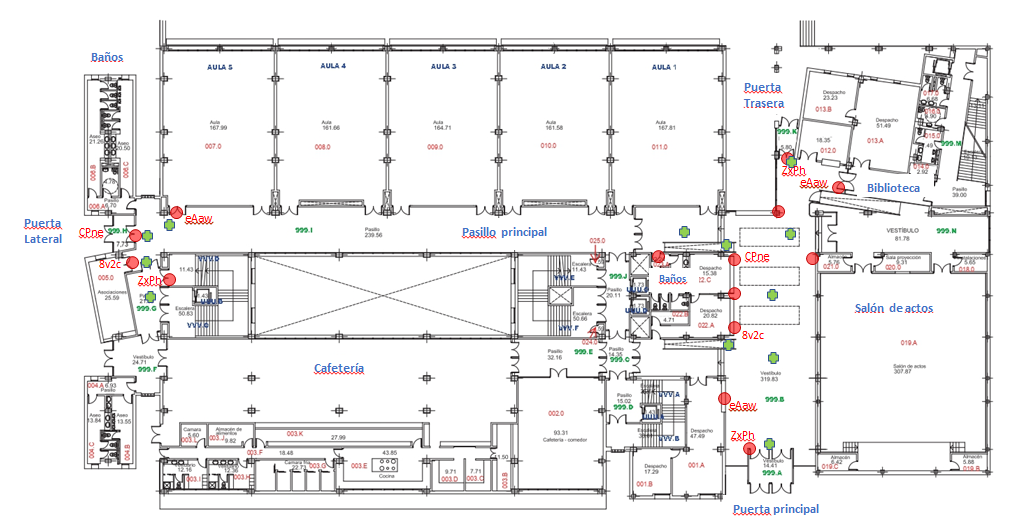
\includegraphics[width=1\textwidth]{Imagenes/Descripciondeltrabajo/mapa_mediciones_plantabaja}
	\caption{Mapa de la planta baja de la Facultad de Informática con la ubicación de los beacons (rojo) y los puntos de medición (verde). }
	\label{fig:medidasPBaja}
\end{figure}


A continuación exponemos las conclusiones obtenidas tras el estudio de los resultados:
\begin{itemize}
	\item Los \textit{beacons} no deben situarse demasiado cerca ya que las señales interfieren entre sí y alteran las distancias no pudiendo distinguir cuál es el \textit{beacon} más cercano. Por este motivo, hemos acordado no poner, por el momento, balizas en los baños ya que, tanto en la primera planta como en la planta baja, se encuentran en zonas repletas de puntos de interés. Para informar de la presencia de los baños y otras zonas de interés se desarrollará una funcionalidad que al pasar cerca de ellos te avisará de su presencia.
	
	\item En lugares diáfanos, como el \textit{hall}, la señal de los \textit{beacons} fluye con mayor libertad ya que no se encuentra con obstáculos. Es por esto, que deben situarse a mayor distancia entre sí. Uno de los problemas que se ha derivado de este hecho es cómo cubrir dicho espacio. Inicialmente colocamos una baliza en conserjería, otra en la intersección superior con el pasillo principal, otra en la intersección inferior con el pasillo que conduce a cafetería y otra enfrente para indicar la entrada al salón de actos (ver Figura \ref{fig:medidasPBaja}). Tras numerosas mediciones, la solución que proponemos es colocar las balizas de modo que una pueda servir para cubrir dos o más puntos de interés. Consecuentemente, hemos suprimido el \textit{beacon} de conserjería y hemos dejado exclusivamente el de las intersecciones ya que la inferior está muy próxima a la ventanilla de conserjería y puede reutilizarse para los dos puntos clave, y hemos desplazado un poco hacia arriba el \textit{beacon} del salón de actos para que sirva tanto para marcar dicho destino como para marcar la esquina superior que conduce hacia la biblioteca. En la Figura \ref{fig:beaconsPBaja} se puede ver el resultado final.
	
	\item Hemos hecho pruebas con los \textit{beacons} sobre distintas superficies y hemos comprobado que efectivamente el material puede alterar la señal. Particularmente, en el caso de las mediciones de la puerta lateral del edificio (lado izquierdo del mapa) hemos colocado el \textit{beacon} CPne justo encima de la puerta, en un bisel metálico que sobresale. El resultado ha sido que la señal de la baliza se proyecta con mayor intensidad, dando lugar a que la distancia estimada sea menor. Es decir, la aplicación sugiere que CPne está más cerca de lo que en realidad está. Tras esto, hemos concluido que lo óptimo es poner los \textit{beacons} sobre las mismas superficies, a ser posible no metálicas, y a la misma altura para que estén en igualdad de condiciones. 
	
	\item La última puntualización que hemos hecho tras las mediciones es que los \textit{beacons} de las intersecciones deben situarse en un punto lo más neutro posible ya que, al menos, se puede llegar desde dos puntos distintos y la señal se debe recibir de manera simétrica. 
\end{itemize}




\begin{figure}[t]
	\centering
	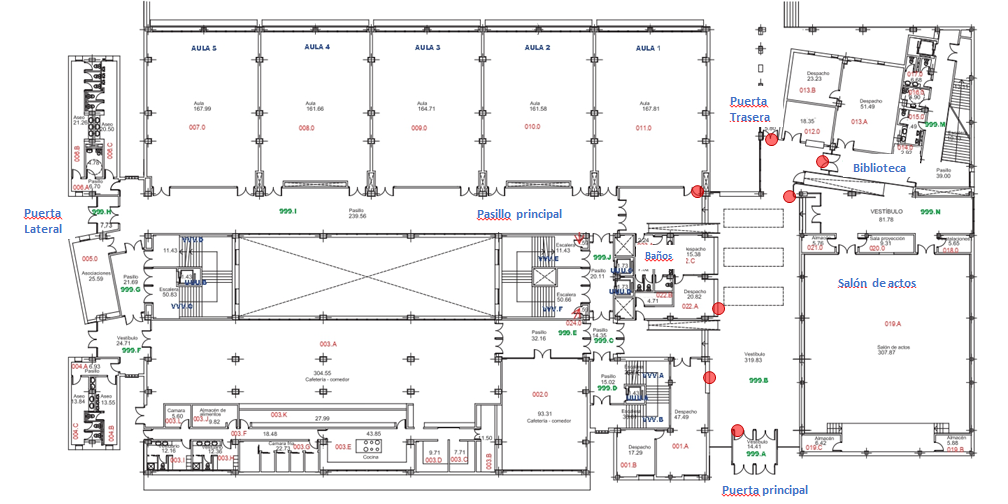
\includegraphics[width=1\textwidth]{Imagenes/Descripciondeltrabajo/beacons_plantabaja_final}
	\caption{Mapa de la planta baja de la Facultad de Informática con la ubicación definitiva de los beacons (rojo) en el hall. }
	\label{fig:beaconsPBaja}
\end{figure}

Este estudio no ha sido todo lo extenso que nos hubiese gustado debido al cierre de la Facultad de Informática a causa del COVID-19.

En el próximo apartado veremos cómo queda reflejado todo el mapeo visto en la Sección \ref{sec:mapeo}.

\section{Representación del mapeo en los XML}
\label{sub:mapeo_xml}
Todo nuestro mapeo se representa en ficheros XML que hemos sacado fuera de la aplicación (se encuentran en una carpeta llamada xml\_modif). En ellos hemos seguido el sistema de divisiones y estructuración del proyecto de TFG \textit{Generador interactivo de instrucciones de guía sobre plataformas móviles} \citep{TFGguia}, este permite que se puedan incluir
de manera sencilla las diferentes plantas del edificio y es un método genérico, lo que facilita que pueda ser empleado también por otros edificios. El sistema descrito se compone de ficheros de dos tipos:

\textbf{Edificio.xml:} En este archivo se guarda la información relativa a la estructura del edificio, es decir, se indican las distintas plantas y el archivo xml asociado a cada una de ellas. A continuación detallamos el significado de cada campo y vemos un ejemplo de la estructura del archivo.

\begin{itemize}
	\item \textit{nombre:} Nombre representativo de la planta que estemos implementando. En el ejemplo se ha utilizado el valor \textit{plantabaja} y \textit{planta1}.
	
	\item \textit{archivo:} Nombre del fichero xml de la planta en cuestión. No es necesario añadir la extensión .xml. En el ejemplo lo hemos llamado \textit{plantabajaarchivo} y \textit{planta1archivo}.
\end{itemize}

%\begin{figure}[t]
%	\centering
%	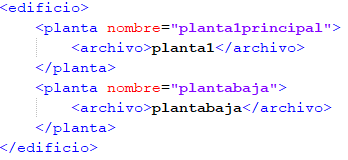
\includegraphics[width=0.7\textwidth]{Imagenes/Descripciondeltrabajo/edificioXML}
%	\caption{Ejemplo de un archivo con la misma estructura que edificio.xml.}
%	\label{fig:xmledificio}
%\end{figure}


\lstinputlisting[language=XML]{Imagenes/Descripciondeltrabajo/edificio.xml}

%\begin{figure}[t]
%	\centering
%	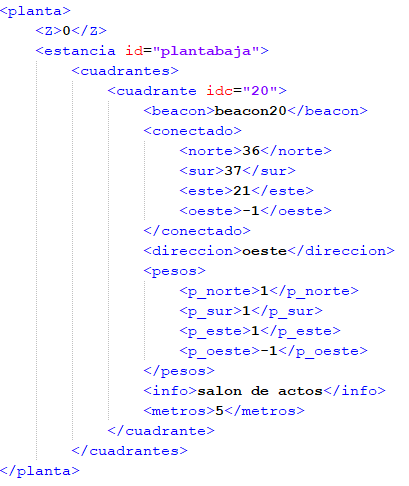
\includegraphics[width=0.7\textwidth]{Imagenes/Descripciondeltrabajo/plantaXML}
%	\caption{Ejemplo de un archivo que detalla la estructura de una planta.}
%	\label{fig:xmlplanta}
%\end{figure}

\textbf{NombreFichero.xml:} Se corresponde con el archivo propio de cada planta. Cada planta incluye un valor que indica el número de planta en el que nos encontramos y un identificador de estancia que da nombre a la planta y que agrupa al conjunto de cuadrantes que la forman. A su vez, cada cuadrante contiene un identificador único, el nombre del \textit{beacon} asociado, información sobre los cuadrantes colindantes, la posición en el cuadrante donde se encuentra el punto de interés (norte, sur, este u oeste), información sobre los pesos que tiene cada una de sus conexiones (cuya utilidad se presenta en la Sección \ref{sub:rutaOptima}), información relevante del cuadrante y la medida en metros del mismo. A continuación detallamos el significado de cada campo y vemos un ejemplo de la estructura del archivo.

\begin{itemize}
	\item \textit{Z:} Indica el número de planta. En el ejemplo le hemos dado el valor $0$.
	
	\item \textit{id:} Se corresponde con el nombre de la planta en la que nos encontramos. En el ejemplo la hemos llamado \textit{plantabaja}.
	
	\item \textit{idc:} Hace referencia al identificador único de cada cuadrante. En el ejemplo le hemos dado el valor $20$.
	
	\item \textit{beacon:} Hace referencia al identificador de la baliza asociada a dicho cuadrante. En el ejemplo le hemos dado el valor \textit{beacon0}.
	
	\item \textit{conectado:} Indica los identificadores de los cuadrantes colindantes por los cuatro puntos cardinales. El valor $-1$ representa la pared. Este campo ha sido reutilizado de trabajos anteriores ya que resulta clave para establecer una red de cuadrantes que nos permita generar una ruta válida pasando a través de ellos.
	
	\item \textit{posdestino:} Nos indica en qué posición del cuadrante está situado el punto de interés. En nuestro caso es el salón de actos, correspondiente al cuadrante $0$, como se puede ver en la Figura \ref{fig:cuadrantesPbaja} el salón de actos se sitúa al lado derecho del cuadrante (oeste)\footnote{La nomenclatura se establece con el sur en la parte de arriba, el oeste a la derecha, el norte abajo y el este a la izquierda del cuadrante.}.
	
	\item \textit{pesos:} Para cada una de las conexiones del cuadrante se establece el peso de dicha conexión. Esto será de gran utilidad pues el algoritmo utilizado para el cálculo de la ruta es el algoritmo de \textit{Dijkstra}. Los detalles pueden verse en la Sección \ref{sub:rutaOptima}. Los pesos negativos se asignan a conexiones inexistentes.
	
	\item \textit{info:} Este campo contiene la información relevante del cuadrante. La utilidad e importancia de este campo radica en informar al usuario, si lo desea, de qué hay a su paso por la ruta hasta el destino seleccionado. Esta idea nació tras la reunión en la ONCE en la que nos acercamos mucho a las necesidades de nuestros usuarios. En el ejemplo le hemos dado el valor \textit{salon de actos}.
	
	\item \textit{metros:} Este campo contiene la medida en metros del cuadrante lo que aporta mucha precisión a las instrucciones. En el ejemplo le hemos dado el valor $5$.
\end{itemize}


\lstinputlisting[language=XML]{Imagenes/Descripciondeltrabajo/planta.xml}

